\pdfminorversion=7
\documentclass[11pt]{report}

\usepackage[a4paper,margin=1in]{geometry}
\usepackage{amsmath,amssymb,mathtools}
\usepackage{graphicx}
\usepackage{booktabs}
\usepackage{hyperref}
\usepackage{xcolor}
\usepackage{pdfpages}

\hypersetup{
  colorlinks=true,
  linkcolor=blue!60!black,
  citecolor=blue!60!black,
  urlcolor=blue!60!black
}

\graphicspath{{figures/}{figures/graphs/}}

\newcommand{\dd}{\mathrm{d}}
\newcommand{\ii}{\mathrm{i}}
\newcommand{\eps}{\varepsilon}
\newcommand{\slashp}[1]{\not{#1}}
\newcommand{\kgone}{k_{g_1}}
\newcommand{\kgtwo}{k_{g_2}}
\newcommand{\Axi}{A_\xi}
\newcommand{\order}[1]{\mathcal{O}\!\left(#1\right)}
\newcommand{\Hamp}{\mathcal{H}}
\newcommand{\Iorig}{\mathcal{I}_{\mathrm{orig}}}
\newcommand{\ICTone}{\mathcal{I}_{C_1}}
\newcommand{\ICTtwo}{\mathcal{I}_{C_2}}

\title{Issues With Dario's Collinear Counterterms\\
for the Two-Loop \(q\bar q\to HHH\) Amplitude}
\author{pygloop qqbar\_nX implementation notes}
\date{\today}

\begin{document}
\maketitle

\tableofcontents

\chapter*{Author-Correction Note}
\addcontentsline{toc}{chapter}{Author-Correction Note}

After this note was first written, Dario Kermanschah confirmed that the
denominator displayed in the published Eqs.~(12)--(13) contains a typo: the
auxiliary propagators must be built from the adjacent gluon momenta
\(k_{g_1}\) and \(k_{g_2}\), not from the light-bridge momentum \(k_1\).  In
the notation used below, the corrected denominators are therefore
\[
  \Axi(k_{g_i})=(k_{g_i}-\xi)^2-\xi^2,
\]
not \(\Axi(k_1)\).  The current \texttt{qqbar\_nX} implementation has been
updated accordingly by splitting the relevant collinear gluon edge and routing
the new massive auxiliary segment as \(k_{g_i}-\xi\).  The severe
soft-collinear enhancement diagnosed in this note is consequently best read as
a diagnosis of the pre-correction \(k_1-\xi\) implementation, not of the
corrected counterterm.

\chapter{Context and Setup}

The process considered here is the two-loop amplitude
\[
  d(p_1)\,\bar d(p_2)\longrightarrow H(p_3)\,H(p_4)\,H(p_5),
\]
where the three Higgs bosons couple to a massive top-quark loop and the
massive loop is connected to the external massless quark line by two gluons.
The local initial-state collinear counterterms are those of
Kermanschah's construction in Ref.~\cite{Kermanschah:2026}.
The implementation discussed here is the one in the \texttt{qqbar\_nX}
process of \texttt{pygloop}.

The DOT file used for the representative topology plots is the final-state
symmetrized process generated by \texttt{qqbar\_nX}. It contains four original
graphs, grouped into two canonical topologies, and the two ISR collinear
counterterms attached to each original graph. The figures were produced from a
GammaLoop state in which this DOT file was loaded and then exported with
\texttt{save dot}; running \texttt{just draw} in that exported state produced
the PDFs included in this note.

\begin{figure}[htbp]
  \centering
  \begin{minipage}{0.31\textwidth}
    \centering
    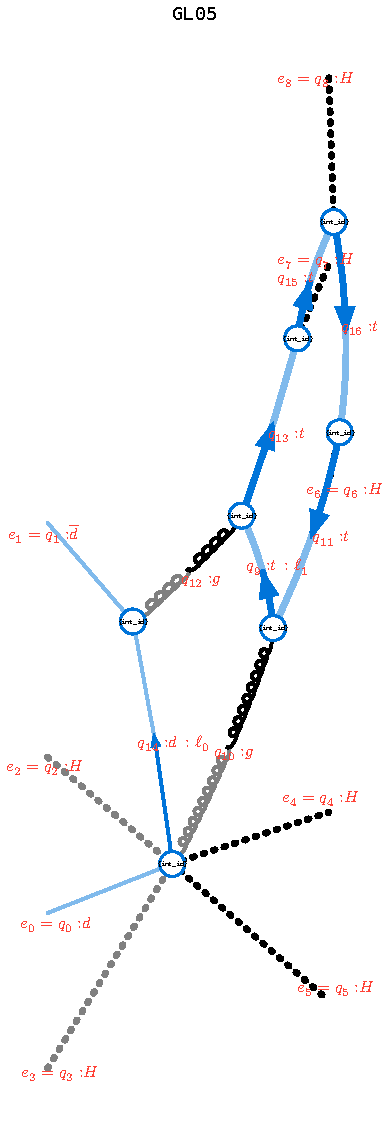
\includegraphics[width=\linewidth,height=0.155\textheight,keepaspectratio]{GL05.pdf}\\
    \small GL05
  \end{minipage}
  \hfill
  \begin{minipage}{0.31\textwidth}
    \centering
    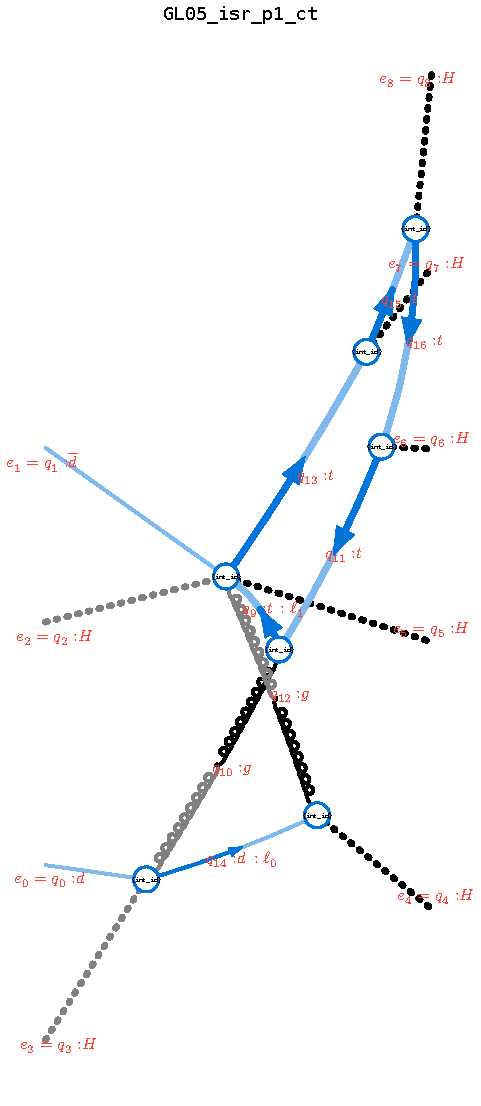
\includegraphics[width=\linewidth,height=0.155\textheight,keepaspectratio]{GL05_isr_p1_ct.pdf}\\
    \small GL05 \(p_1\)-collinear CT
  \end{minipage}
  \hfill
  \begin{minipage}{0.31\textwidth}
    \centering
    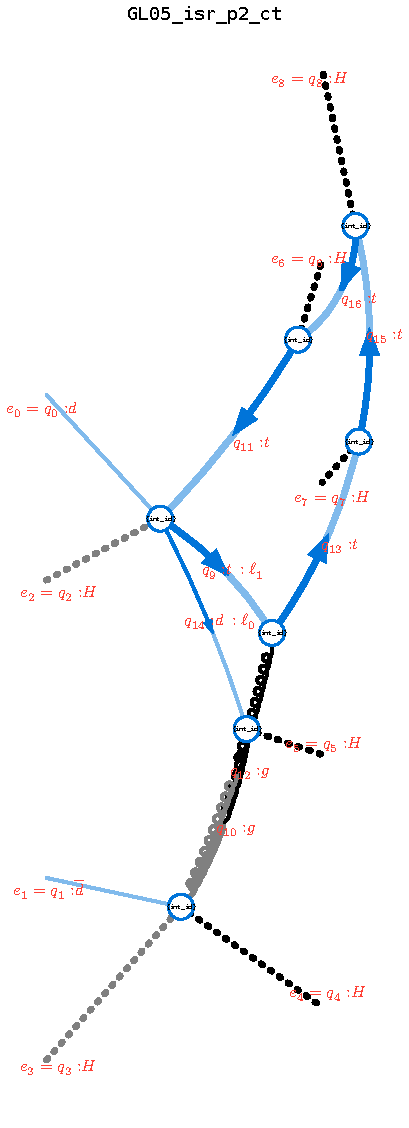
\includegraphics[width=\linewidth,height=0.155\textheight,keepaspectratio]{GL05_isr_p2_ct.pdf}\\
    \small GL05 \(p_2\)-collinear CT
  \end{minipage}

  \vspace{1.0em}

  \begin{minipage}{0.31\textwidth}
    \centering
    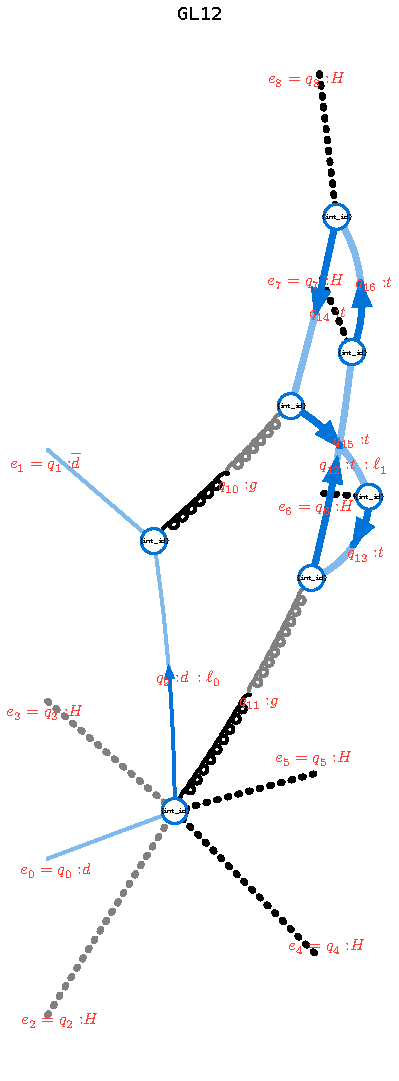
\includegraphics[width=\linewidth,height=0.155\textheight,keepaspectratio]{GL12.pdf}\\
    \small GL12
  \end{minipage}
  \hfill
  \begin{minipage}{0.31\textwidth}
    \centering
    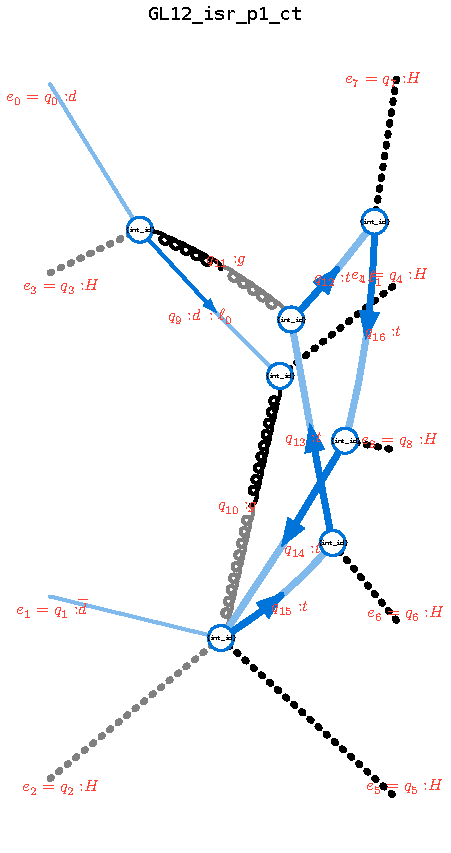
\includegraphics[width=\linewidth,height=0.155\textheight,keepaspectratio]{GL12_isr_p1_ct.pdf}\\
    \small GL12 \(p_1\)-collinear CT
  \end{minipage}
  \hfill
  \begin{minipage}{0.31\textwidth}
    \centering
    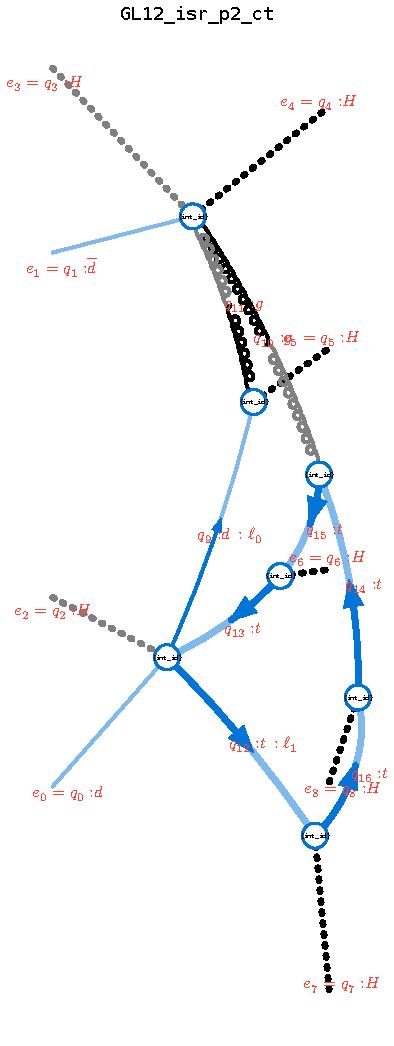
\includegraphics[width=\linewidth,height=0.155\textheight,keepaspectratio]{GL12_isr_p2_ct.pdf}\\
    \small GL12 \(p_2\)-collinear CT
  \end{minipage}
  \caption{Two representative final-state-symmetrized original topologies and
  their local ISR collinear counterterms. The full GammaLoop drawing grid is
  included in Appendix~\ref{app:drawings}.}
  \label{fig:topologies}
\end{figure}

\chapter{Four-Dimensional Local Representation}

\section{Light-line denominators}

Only the light massless bridge is needed to expose the endpoint problem. We
write the loop momentum on the light quark bridge as
\[
  k_1 \equiv K_0 ,
\]
with the two adjacent gluon momenta denoted by \(\kgone\) and \(\kgtwo\).
For the scaling discussion we use the convention
\[
  \kgone = k_1-p_1,\qquad
  \kgtwo = -k_1-p_2.
\]
The sign convention is not important for the power counting; what matters is
that \(\kgone\) becomes longitudinal and on shell in the \(p_1\)-collinear
soft endpoint, while \(\kgtwo\) becomes longitudinal and on shell in the
\(p_2\)-collinear soft endpoint.

Suppressing all massive-loop denominators, the relevant original light part is
\[
  D_{\mathrm{orig}} =
    k_1^2\,\kgone^2\,\kgtwo^2 .
  \label{eq:orig-light-den}
\]
The exact-\(\xi\) counterterm topology replaces the non-local light
denominator by the auxiliary denominator
\[
  \Axi(k_1) \equiv (k_1-\xi)^2-\xi^2 = k_1^2-2\,\xi\cdot k_1.
  \label{eq:axi}
\]
The two counterterm light denominator structures used in the DOT files are
\[
  D_{C_1} = k_1^2\,\kgone^2\,\Axi(k_1),\qquad
  D_{C_2} = k_1^2\,\Axi(k_1)\,\kgtwo^2 .
  \label{eq:ct-denominators}
\]
The helper external momenta are only used to realize \(\Axi\) as an ordinary
GammaLoop denominator. In the exact-\(\xi\) DOT strategy, the original graphs
have the helper half-edges marked as dummy. In the \(C_1\) counterterm only
the \(Q(2),Q(4)\) helper pair is active, and in the \(C_2\) counterterm only
the \(Q(3),Q(5)\) helper pair is active. The inactive pair is dummy. The mass
override of the shifted auxiliary edge is \(\xi^2\), represented by the
corresponding active helper momentum squared, so the construction remains
\(\xi\)-generic.

\section{Numerators and the observed mismatch}

The original numerator contains the massless bridge spinor chain
\[
  N_{\mathrm{orig}}
  =
  \bar v(p_2)\,\gamma_{\mu_2}\,\slashp{k_1}\,\gamma_{\mu_1}\,u(p_1)\,
  \Hamp^{\mu_1\mu_2}(\kgone,\kgtwo;\{p_H\}),
  \label{eq:orig-num}
\]
where \(\Hamp^{\mu_1\mu_2}\) is the massive top-loop tensor with three Higgs
insertions. The counterterm numerators are inserted as graph-global tensor
network numerators in the DOT file; edge and vertex numerators inside the CT
topology are set to one. No finite routing-ratio factors are inserted in the
numerator. The relevant collinear-projected part of the first CT is
schematically
\[
  N_{C_1}
  \sim
  \bar v(p_2)\,\Gamma_{C_1}^{\mu_2}(p_1,p_2,k_1,\xi)\,u(p_1)\,
  \kgone^{\mu_1}\,
  \Hamp_{\mu_1\mu_2}(\kgone,\kgtwo;\{p_H\}),
  \label{eq:ct1-num}
\]
with an analogous expression for \(C_2\) containing \(\kgtwo^{\mu_2}\). The
crucial point is that the original spinor chain has an explicit soft
\(\slashp{k_1}\), while the projected CT numerator can remain finite in the
soft-collinear endpoint unless a Ward identity kills
\(\kgone^{\mu_1}\Hamp_{\mu_1\mu_2}\) or
\(\kgtwo^{\mu_2}\Hamp_{\mu_1\mu_2}\).

\section{\(p_1\)-soft-collinear scaling}

Take
\[
  p_1 = E(1,0,0,1),\qquad
  p_2 = E(1,0,0,-1),\qquad
  \xi = p_1+p_2 = (2E,0,0,0),
\]
and approach the \(p_1\)-soft-collinear endpoint with
\[
  k_1 = E\lambda(1,1,0,1),\qquad \lambda\to 0^+ .
\]
Then
\begin{align}
  k_1^2 &= -E^2\lambda^2,\\
  \kgone^2 &= (k_1-p_1)^2 = -E^2\lambda^2,\\
  \kgtwo^2 &= (-k_1-p_2)^2 = E^2(4\lambda-\lambda^2)
             = \order{\lambda},\\
  \Axi(k_1) &= k_1^2 -2\xi\cdot k_1
             = -4E^2\lambda+\order{\lambda^2}.
\end{align}
Hence
\[
  D_{\mathrm{orig}}\sim \lambda^5,\qquad
  D_{C_1}\sim \lambda^5,\qquad
  D_{C_2}\sim \lambda^5 .
\]
The denominators alone do not distinguish the original from the singular CT.
The mismatch is instead
\[
  N_{\mathrm{orig}}\sim \lambda,
  \qquad
  N_{C_1}\sim \lambda^0
  \quad\text{if}\quad
  \kgone^{\mu_1}\Hamp_{\mu_1\mu_2}\not\to 0 .
\]
Therefore the direct four-dimensional local objects scale as
\[
  |\Iorig|\sim \lambda^{-4},\qquad
  |\ICTone|\sim \lambda^{-5},\qquad
  |\ICTtwo|\sim \lambda^{-4},
  \label{eq:4d-scaling-p1}
\]
with the total dominated by \(C_1\). The \(p_2\)-soft-collinear endpoint is
the beam-exchanged version:
\[
  |\Iorig|\sim \lambda^{-4},\qquad
  |\ICTone|\sim \lambda^{-4},\qquad
  |\ICTtwo|\sim \lambda^{-5}.
  \label{eq:4d-scaling-p2}
\]

The direct \texttt{pygloop} four-dimensional evaluator, using the same
graph-level numerators and denominator definitions as the emitted DOT file,
finds the following fitted powers:
\begin{center}
\begin{tabular}{lcccc}
\toprule
Approach & original & \(C_1\) & \(C_2\) & total\\
\midrule
\(p_1\)-soft-collinear & \(-4.000\) & \(-5.000\) & \(-4.000\) & \(-5.000\)\\
\(p_2\)-soft-collinear & \(-4.000\) & \(-4.000\) & \(-4.999\) & \(-4.999\)\\
\bottomrule
\end{tabular}
\end{center}
where the entries mean \(|I|\propto \lambda^{p}\). This confirms that the
problem is already present before any CFF subtleties are introduced.

\chapter{Three-Dimensional CFF Representation}

\section{Schematic CFF weight}

After applying the causal-flow/energy-residue representation, a local
three-dimensional contribution has the schematic form
\[
  W(\vec K_0,\vec K_1)
  =
  J(\vec K_0,\vec K_1)\,
  \sum_{\omega\in\Omega}
  \frac{N_\omega(\vec K_0,\vec K_1)}
       {\prod_{F\in\mathcal F_\omega} F_\omega(\vec K_0,\vec K_1)} .
  \label{eq:cff-weight}
\]
Here \(J\) is the mapping Jacobian and the \(F_\omega\) are the causal
energy-surface denominators for a given orientation \(\omega\). The exact
power of an endpoint scan depends on which cube variable is used to approach
the surface and on the selected loop-momentum basis. What is robust in the
observed scans is the hierarchy: the CT assigned to the soft-collinear beam
is one power worse than the corresponding original graph.

For the endpoint scan used in the GammaLoop-rich-output and custom-CFF
checks, the cube variables were taken as
\begin{equation}
  \begin{aligned}
  x(\Delta)=
  \bigl(&
  \Delta,\; 0.8941729073613068,\; 1-\Delta,\;
  0.05523624797827975,\\
  &0.7717783989563521,\;0.4505175649210359
  \bigr),
  \qquad \Delta\to 0^+ .
  \end{aligned}
  \label{eq:endpoint-scan}
\end{equation}
With threshold subtraction disabled, the observed three-dimensional
GammaLoop/CFF weights scale as
\[
  |W_{\mathrm{orig}}|\sim \Delta^{-1},\qquad
  |W_{C_i}|\sim \Delta^{-2},\qquad
  |W_{\mathrm{tot}}|\sim \Delta^{-2},
  \label{eq:3d-scaling}
\]
for the CT \(C_i\) associated with the beam being approached. The powers are
softer than the direct four-dimensional density because the CFF residues and
the unit-cube mapping already include part of the spatial measure and energy
Jacobian. They nevertheless reproduce the same structural failure: the local
CT has one more inverse endpoint power than the original contribution it is
supposed to subtract.

\section{Denominator origin of the residual growth}

Near the soft-collinear endpoint, the CFF energy surfaces generated by the
light bridge inherit the same small scales as the four-dimensional
denominators:
\[
  E_{k_1}\sim \Delta,\qquad
  E_{\kgone}\sim \Delta,\qquad
  \Axi \sim \Delta .
\]
The original graph contains the soft bridge numerator suppression from
\(\slashp{k_1}\). The CT topology has the same small CFF surfaces after the
auxiliary replacement, but its projected numerator contains the longitudinal
massive-loop contraction \(k_{g_i}\cdot\Hamp\). If that contraction is finite
instead of soft, the CFF weight keeps one additional inverse power. This is
the three-dimensional version of Eqs.~\eqref{eq:4d-scaling-p1} and
\eqref{eq:4d-scaling-p2}.

\chapter{Ward-Identity Rescue Attempt}

\section{Why the Ward identity should help}

The reason a careful routing could in principle cure the problem is the
massive-loop Ward identity. For a gluon with momentum \(k_g\) attached to a
fermion line with momentum \(q\),
\[
  \slashp{k_g}
  =
  \bigl(\slashp{q}+\slashp{k_g}-m_t\bigr)
  -
  \bigl(\slashp{q}-m_t\bigr)
  =
  S^{-1}(q+k_g)-S^{-1}(q).
  \label{eq:ward-local}
\]
When all insertions of a longitudinal gluon into a closed fermion loop are
summed with a common loop-momentum routing, the inverse propagator differences
in Eq.~\eqref{eq:ward-local} telescope:
\[
  k_g^\mu
  \sum_{\mathrm{insertions}}\Hamp_{\mu\nu}^{(\mathrm{insertion})}
  =
  0.
  \label{eq:ward-loop}
\]
In the \(p_1\)-soft-collinear endpoint,
\[
  \kgone \longrightarrow -p_1,\qquad \kgone^2\longrightarrow 0,
\]
so the gluon momentum contracted into the CT numerator becomes an on-shell
longitudinal momentum. If Eq.~\eqref{eq:ward-loop} were realized locally
inside the grouped integrand, then
\[
  \kgone^{\mu_1}
  \sum_{\mathrm{Ward\ orbit}}\Hamp_{\mu_1\mu_2}
  =
  \order{\lambda},
\]
and the first CT would scale like
\[
  |\ICTone^{\mathrm{Ward\ summed}}|
  \sim
  \lambda^{-4}
\]
instead of \(\lambda^{-5}\). The same argument applies to \(C_2\) in the
\(p_2\)-soft-collinear endpoint. This is why restoring the local Ward orbit
was a plausible rescue strategy.

\section{Routing strategy that was implemented}

The routing attempt used the following explicit strategy.

\begin{enumerate}
  \item Set the defining light loop momentum \(K_0\) by assigning
  \(\texttt{lmb\_id=0}\) to the massless bridge edge between the two gluon
  insertions. This makes \(k_1=K_0\) directly, so the collinear approach can
  be made with \(K_0\) parallel to the beam direction.

  \item Use the exact-\(\xi\) helper-edge topology for the CTs. The original
  graphs carry the same helper external half-edges, but all helper edges are
  dummy there, so the original graph is independent of \(Q(2),Q(3),Q(4),Q(5)\).
  The \(p_1\)-collinear CT uses the active pair \(Q(2),Q(4)\) and is
  independent of \(Q(3),Q(5)\). The \(p_2\)-collinear CT uses the active pair
  \(Q(3),Q(5)\) and is independent of \(Q(2),Q(4)\). This lets all active
  helpers be set directly to the same chosen \(\xi\).

  \item For the Ward-complete test, disable final-state symmetrization and
  retain the full set of Higgs orderings. Put all original graphs and all CTs
  into a single \(\texttt{group\_id}\), so the local sum has access to the full
  Ward orbit rather than only a final-state-symmetrized subset.

  \item Pin the heavy-loop momentum \(K_1\) by assigning \(\texttt{lmb\_id=1}\)
  to a heavy top edge adjacent to a fixed labelled Higgs insertion. In the
  exact-\(\xi\) external ordering the physical Higgs labels are shifted by the
  helper externals, so the raw anchor \(H_2\) is represented as the emitted
  external \(H_6\). The selected edge is one of the two heavy-loop edges
  adjacent to this labelled insertion, with the side chosen canonically from
  the neighboring labels and the orientation chosen consistently with the
  fermion flow.

  \item Keep both fermion-flow orientations, i.e. for every Higgs ordering
  include the orientation in which the anchored momentum flows along the
  fermion flow and the orientation in which it flows against it. This is
  needed because the Ward sum telescopes only after the routed massive-loop
  momenta are aligned consistently across the orbit.
\end{enumerate}

This routing improves the formal conditions for Eq.~\eqref{eq:ward-loop}, but
the direct four-dimensional scans still show the same endpoint hierarchy:
the soft-collinear CT scales one power worse than the original. The conclusion
from this check is that the current grouped integrand still does not realize
the required local Ward cancellation strongly enough to remove the endpoint
growth.

\chapter{Current Interpretation}

The endpoint issue is not caused by a missing threshold subtraction in the
four-dimensional object, nor by an explicit ratio inserted in the numerator.
It is already visible in the purely local tensor numerator and the intended
denominator structure. The problematic ingredients are:
\begin{itemize}
  \item the CT denominator retains the two small light denominators
  \(k_1^2\) and \(k_{g_i}^2\) and replaces the other light denominator by
  \(\Axi\sim \lambda\);
  \item the original graph has a soft bridge numerator
  \(\slashp{k_1}\sim\lambda\);
  \item the CT numerator has a longitudinal contraction
  \(k_{g_i}^{\mu}\Hamp_{\mu\nu}\) that is finite unless the local Ward sum is
  realized;
  \item the final-state-symmetrized minimal groups do not contain the full
  massive-loop Ward orbit, and the Ward-complete routing test has not yet
  produced the required local telescoping cancellation.
\end{itemize}

Thus the soft-collinear endpoint has the structure
\[
  \frac{N_{\mathrm{orig}}\sim\lambda}
       {D_{\mathrm{orig}}\sim\lambda^5}
  \quad\text{versus}\quad
  \frac{N_{C_i}\sim 1}
       {D_{C_i}\sim\lambda^5}.
\]
In 3D CFF variables this same mismatch appears as a one-power stronger
endpoint growth of the CT weight.

\chapter{Idea: Symmetrized Collinear Counterterms}

A possible way forward is to modify the local CT by a symmetrization that
keeps its integrated value zero. Let \(\Delta_i(\ell)\) denote one of the
local collinear CT integrands, where \(\ell\) denotes all loop variables. The
current construction has
\[
  \int \dd\ell\, \Delta_i(\ell)=0
\]
after the corresponding integrated contribution is accounted for in the
subtraction scheme. Consider a finite set \(S\) of measure-preserving maps
\(\sigma\) acting on the local loop variables, external-Higgs labels,
heavy-loop orientation, or beam/auxiliary-\(\xi\) assignments. Define
\[
  \Delta_i^{\mathrm{sym}}(\ell)
  =
  \frac{1}{|S|}
  \sum_{\sigma\in S}
  J_\sigma(\ell)\,
  \Delta_i\!\left(\sigma(\ell)\right),
  \label{eq:sym-ct}
\]
where \(J_\sigma\) is the Jacobian of the transformation. If the maps are
bijective and cover the same integration domain, then
\[
  \int \dd\ell\,\Delta_i^{\mathrm{sym}}(\ell)
  =
  \frac{1}{|S|}
  \sum_{\sigma\in S}
  \int \dd\ell_\sigma\,\Delta_i(\ell_\sigma)
  =
  0.
  \label{eq:sym-zero}
\]
The hope is to choose \(S\) so that the finite longitudinal pieces of
\(k_{g_i}\cdot\Hamp\) cancel locally in the soft-collinear endpoint, while the
strict collinear limit that the CT is designed to subtract is left unchanged.

Natural candidates for \(S\) include:
\begin{itemize}
  \item permutations of the identical Higgs insertions on the massive loop;
  \item reversal of the massive-loop orientation, paired with the corresponding
  ordered Higgs labels;
  \item exchange of the two sides of the light bridge, paired with
  \(p_1\leftrightarrow p_2\) and
  \((Q(2),Q(4))\leftrightarrow(Q(3),Q(5))\);
  \item a Ward-orbit average over all insertions of the longitudinal gluon on
  the massive loop, written as an explicitly symmetrized CT numerator rather
  than relying on the graph grouping alone.
\end{itemize}

This would not be a change in the integrated subtraction if the maps are
implemented as exact changes of variables. It would instead redistribute the
zero-integral CT locally to make the endpoint behavior compatible with the
massive-loop Ward identity.

\appendix

\chapter{Full GammaLoop Drawing Grid}
\label{app:drawings}

The following page is the direct output of running \texttt{just draw} in the
GammaLoop \texttt{save dot} export of the final-state-symmetrized process.

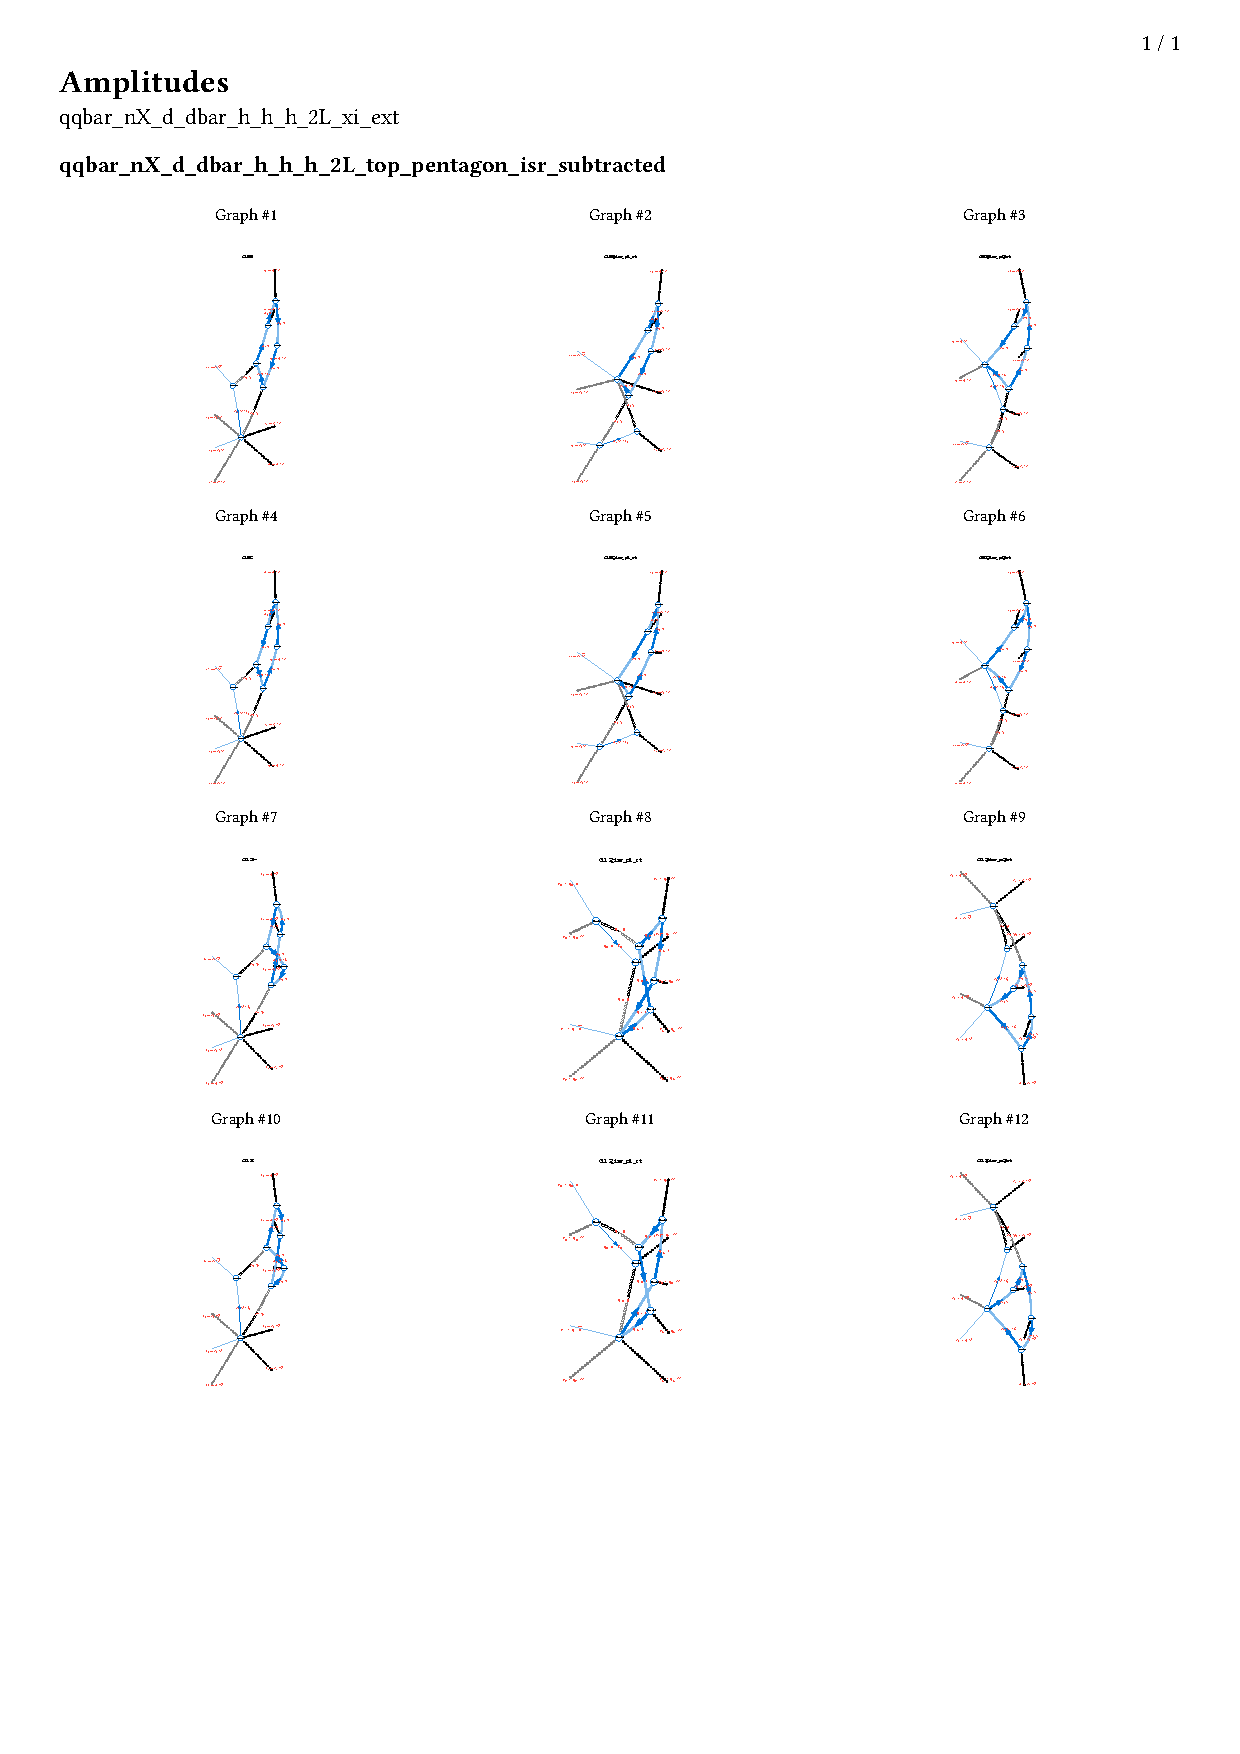
\includepdf[pages=-,pagecommand={}]{figures/symmetrized_graphs_and_cts.pdf}

\begin{thebibliography}{9}
\bibitem{Kermanschah:2026}
Kermanschah et al.,
\emph{Local initial-state collinear subtraction for loop amplitudes},
\href{https://arxiv.org/abs/2603.03169}{arXiv:2603.03169}.
\end{thebibliography}

\end{document}
